% =====================================================================
% EJEMPLO: Guía del estudiante -- Geometría 3° (registro infantil)
% María Mercedes Cantillo · Colegio San Alberto Magno
% ---------------------------------------------------------------------
% Misma estructura que guia-trimestral.tex, adaptada a niños de 8-9 años
% (ver "Grados 3° a 6°" en CLAUDE.md):
%   - hilo conductor: un cuento clásico colombiano (Rafael Pombo, dominio
%     público), contado en nuestra versión y solo en sus partes amables;
%   - oraciones cortas, trato cercano, cada palabra nueva con dibujo;
%   - marco teórico con anécdotas ("¿Sabías que…?"), sin citas textuales;
%   - trabajo manipulativo: dibujar, contar, recortar, caminar el salón.
% =====================================================================
\documentclass[11pt]{article}
\makeatletter\def\input@path{{../estilo/}}\makeatother
\usepackage{mmcantillo}

% ======================== DATOS DE LA GUÍA ============================
\tipodocumento{Guía del estudiante}
\asignatura{Geometría}
\titulo{Formas y caminos a mi alrededor}
\grado{3°}
\periodo{I}
\hiloconductor{El paseo de Rinrín Renacuajo}
% ======================================================================
% DBA: matematicas grado 03 · DBA 6 y DBA 7 (dba/matematicas/grados/grado03.tex)

% Etiqueta redonda para lugares del mapa (R, T, P, C)
\tikzset{lugar/.style={circle, draw, fill=white, thick, inner sep=1.5pt,
  font=\footnotesize\bfseries}}

\begin{document}

\encabezado

% ---------------------------------------------------------------------
% 1. Frase introductoria
% ---------------------------------------------------------------------
% verificado: https://babel.banrepcultural.org/digital/api/collection/p17054coll10/id/2720/download — Cuentos pintados para niños (1867), versos iniciales de «El renacuajo paseador»
\frase{El hijo de Rana, Rinrín Renacuajo, salió esta mañana muy tieso y
muy majo, con pantalón corto, corbata a la moda, sombrero encintado y
chupa de boda.}
{Rafael Pombo, \emph{El renacuajo paseador} (1867)}

% ---------------------------------------------------------------------
% 2. Introducción
% ---------------------------------------------------------------------
\seccion{Introducción}

¡Mira a tu alrededor! La ventana es un rectángulo. El reloj es un
círculo. Tu borrador parece una caja. Las formas están en todas partes.

En este periodo vas a aprender a \textbf{nombrar las formas}, a
\textbf{contar sus partes} y a \textbf{explicar caminos} para llegar de un
lugar a otro.

Te acompañará Rinrín Renacuajo, el personaje del poeta colombiano Rafael
Pombo~\cite{pombo}. En nuestra versión del cuento, Rinrín sale de su charco a pasear
por el barrio. En el camino descubre formas, visita una tienda y tiene
que encontrar el camino de regreso a casa. ¡Vamos con él!

\textbf{Al terminar este periodo podrás:}
\begin{itemize}
  \item nombrar figuras planas y contar sus lados y vértices;
  \item reconocer cuerpos geométricos en los objetos de tu casa y tu colegio;
  \item seguir y dar instrucciones para ir de un lugar a otro.
\end{itemize}

Estos son los aprendizajes que el Ministerio de Educación espera para tu
grado~\cite{mendba}:

\begin{dba}[Grado 3 · DBA 6]
Describe y representa formas bidimensionales y tridimensionales de
acuerdo con las propiedades geométricas.
\end{dba}

\begin{dba}[Grado 3 · DBA 7]
Formula y resuelve problemas que se relacionan con la posición, la
dirección y el movimiento de objetos en el entorno.
\end{dba}

% ---------------------------------------------------------------------
% 3. Marco teórico (en 3°: anécdotas, sin citas textuales)
% ---------------------------------------------------------------------
\seccion{Marco teórico: ¿Sabías que…?}

\subsubsection*{Un libro de formas muy, muy antiguo}
Hace más de 2\,000 años, en la ciudad de Alejandría (Egipto), un maestro
llamado \textbf{Euclides} escribió un libro sobre las formas: los
\emph{Elementos}. Allí explicó qué es un punto, una línea y un triángulo.
¡Todavía hoy se estudia!~\cite{euclides}

\subsubsection*{Una maestra que miraba el cielo}
En esa misma ciudad vivió \textbf{Hipatia}, una de las primeras mujeres
matemáticas de la historia. Enseñaba geometría y estudiaba el movimiento
de las estrellas. Muchos estudiantes viajaban desde lejos para
escucharla~\cite{dzielska}.

\subsubsection*{Las abejas también saben geometría}
Las abejas construyen sus panales con celdas de \textbf{seis lados}. En
el año 2001, el matemático Thomas Hales demostró que los hexágonos dividen una
superficie en partes iguales usando el borde más corto posible. Por eso se piensa
que así las abejas ahorran cera~\cite{hales}.

% ---------------------------------------------------------------------
% 4. Temas
% ---------------------------------------------------------------------
\tema{Figuras planas: lados y vértices}\label{tema:figuras}

\begin{hilo}
Rinrín sale muy elegante de su charco. En la esquina ve una señal de
tránsito, las ventanas de las casas y la rueda de una bicicleta.
«¡Cuántas formas!», dice. «¿Cómo se llamarán?»
\end{hilo}

Las \textbf{figuras planas} son formas que podemos dibujar en una hoja.
Estas son cuatro muy importantes:

\begin{center}
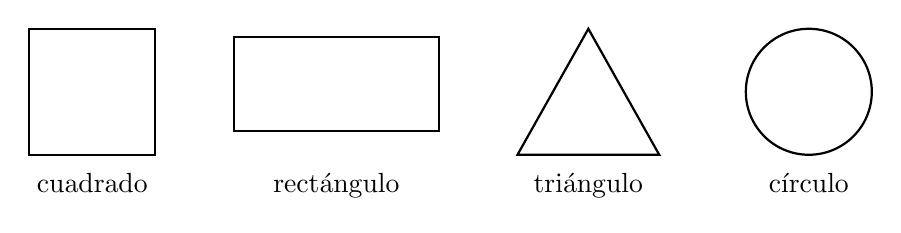
\begin{tikzpicture}[thick, every node/.append style={text height=1.6ex, text depth=0.3ex}]
  \draw (0,0) rectangle (1.6,1.6);          \node[below] at (0.8,-0.1) {cuadrado};
  \draw (2.6,0.3) rectangle (5.2,1.5);      \node[below] at (3.9,-0.1) {rectángulo};
  \draw (6.2,0) -- (8.0,0) -- (7.1,1.6) -- cycle; \node[below] at (7.1,-0.1) {triángulo};
  \draw (9.9,0.8) circle (0.8);             \node[below] at (9.9,-0.1) {círculo};
\end{tikzpicture}
\end{center}

Cada línea del borde de una figura es un \textbf{lado}. El punto donde se
juntan dos lados es un \textbf{vértice}. ¡El círculo no tiene lados rectos
ni vértices!

\begin{center}
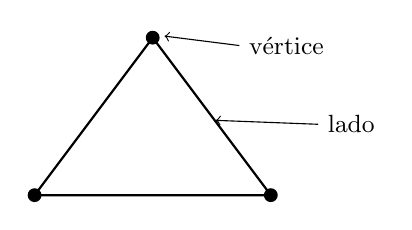
\begin{tikzpicture}[thick]
  \draw (0,0) -- (3,0) -- (1.5,2) -- cycle;
  \foreach \p in {(0,0),(3,0),(1.5,2)} \fill \p circle (2.5pt);
  \draw[->, thin] (2.6,1.9) node[right, font=\small] {vértice} -- (1.65,2.02);
  \draw[->, thin] (3.6,0.9) node[right, font=\small] {lado} -- (2.3,0.95);
\end{tikzpicture}
\end{center}

\begin{ejemplo}[Contar las partes]
El triángulo tiene \textbf{3 lados} y \textbf{3 vértices}. El cuadrado
tiene \textbf{4 lados} y \textbf{4 vértices}. Todos los lados del
cuadrado miden lo mismo; el rectángulo tiene dos lados largos y dos cortos.
\end{ejemplo}

\begin{aplicacion}[Señales de tránsito]
Las señales tienen formas distintas para que los conductores las
reconozcan desde lejos. La señal de \textbf{PARE} tiene 8 lados. La de
\textbf{CEDA EL PASO} es un triángulo. Así, ¡hasta sin leerlas sabemos
qué dicen!
\end{aplicacion}

\begin{preguntas}
\Needspace{11\baselineskip}% enunciado y tabla en la misma página
\pregunta Completa la tabla. Puedes pasar el dedo por el borde para
contar.
\begin{center}
{\renewcommand{\arraystretch}{1.8}
\begin{tabular}{|l|c|c|}
  \hline
  \textbf{Figura} & \textbf{Número de lados} & \textbf{Número de vértices}\\\hline
  Triángulo  & \hspace{2.5cm} & \hspace{2.5cm}\\\hline
  Cuadrado   & & \\\hline
  Rectángulo & & \\\hline
  Círculo    & & \\\hline
\end{tabular}}
\end{center}
\pregunta Busca en tu salón un objeto con forma de rectángulo y otro con
forma de círculo. Dibújalos y escribe su nombre.
\espacio{3.5cm}
\end{preguntas}

\begin{resumen}
\begin{itemize}
  \item Las figuras planas se pueden dibujar en una hoja: cuadrado,
        rectángulo, triángulo y círculo.
  \item Los \textbf{lados} son las líneas del borde; los \textbf{vértices}
        son las esquinas donde se juntan dos lados.
  \item El círculo no tiene lados rectos ni vértices.
\end{itemize}
\end{resumen}

% ---------------------------------------------------------------------
\tema{Cuerpos geométricos}\label{tema:cuerpos}

\begin{hilo}
Rinrín entra a la tienda del barrio. Ve cajas de cereal, latas de
atún, pelotas de colores y conos de helado. «Estas formas no son planas»,
piensa. «¡Se pueden agarrar con las manos!»
\end{hilo}

Los \textbf{cuerpos geométricos} ocupan un lugar en el espacio: tienen
largo, ancho y alto. Algunos tienen solo \textbf{caras planas}, y otros
tienen \textbf{partes curvas} que les permiten rodar.

\begin{center}
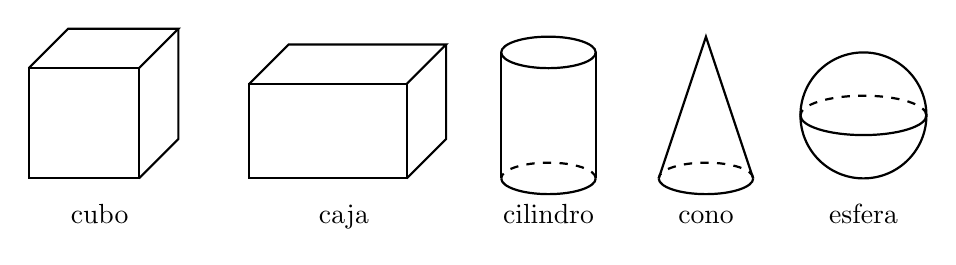
\begin{tikzpicture}[thick, every node/.append style={text height=1.6ex, text depth=0.3ex}]
  % cubo
  \draw (0,0) rectangle (1.4,1.4);
  \draw (0,1.4) -- (0.5,1.9) -- (1.9,1.9) -- (1.4,1.4);
  \draw (1.9,1.9) -- (1.9,0.5) -- (1.4,0);
  \node[below] at (0.9,-0.2) {cubo};
  % caja (prisma rectangular)
  \begin{scope}[xshift=2.8cm]
    \draw (0,0) rectangle (2,1.2);
    \draw (0,1.2) -- (0.5,1.7) -- (2.5,1.7) -- (2,1.2);
    \draw (2.5,1.7) -- (2.5,0.5) -- (2,0);
    \node[below] at (1.2,-0.2) {caja};
  \end{scope}
  % cilindro
  \begin{scope}[xshift=6.6cm]
    \draw (0,1.6) ellipse (0.6 and 0.2);
    \draw (-0.6,1.6) -- (-0.6,0);  \draw (0.6,1.6) -- (0.6,0);
    \draw (-0.6,0) arc (180:360:0.6 and 0.2);
    \draw[dashed] (0.6,0) arc (0:180:0.6 and 0.2);
    \node[below] at (0,-0.2) {cilindro};
  \end{scope}
  % cono
  \begin{scope}[xshift=8.6cm]
    \draw (-0.6,0) -- (0,1.8) -- (0.6,0);
    \draw (-0.6,0) arc (180:360:0.6 and 0.2);
    \draw[dashed] (0.6,0) arc (0:180:0.6 and 0.2);
    \node[below] at (0,-0.2) {cono};
  \end{scope}
  % esfera
  \begin{scope}[xshift=10.6cm]
    \draw (0,0.8) circle (0.8);
    \draw (-0.8,0.8) arc (180:360:0.8 and 0.25);
    \draw[dashed] (0.8,0.8) arc (0:180:0.8 and 0.25);
    \node[below] at (0,-0.2) {esfera};
  \end{scope}
\end{tikzpicture}
\end{center}

\begin{ejemplo}[¿Rueda o no rueda?]
El cubo y la caja tienen solo caras planas: \textbf{no ruedan}. La esfera
es toda curva: \textbf{rueda en cualquier dirección}. El cilindro y el
cono tienen una parte curva y caras planas: ruedan solo si los acuestas.
\end{ejemplo}

\begin{aplicacion}[En la tienda]
Las cajas se pueden poner una encima de otra sin que se caigan, porque
sus caras son planas. Por eso los cereales y los zapatos vienen en cajas.
Las latas, en cambio, son cilindros: ¡si las acuestas, ruedan!
\end{aplicacion}

\begin{preguntas}
\pregunta Une con una línea cada objeto con el nombre de su forma.
\begin{center}
\begin{tabular}{l@{\hspace{3cm}}l}
  una pelota       & cilindro\\[0.6em]
  una lata de atún & cubo\\[0.6em]
  un dado          & esfera\\[0.6em]
  un cono de helado & cono\\
\end{tabular}
\end{center}
\pregunta Trae de tu casa un objeto con forma de caja. Cuenta sus caras
y escribe cuántas tiene. ¿Todas las caras son iguales?
\renglones{2}
\end{preguntas}

\begin{resumen}
\begin{itemize}
  \item Los cuerpos geométricos tienen largo, ancho y alto: cubo, caja,
        cilindro, cono y esfera.
  \item Los cuerpos con solo caras planas no ruedan; los que tienen partes
        curvas pueden rodar.
\end{itemize}
\end{resumen}

% ---------------------------------------------------------------------
\tema{¿Dónde está? Posiciones y caminos}\label{tema:caminos}

\begin{hilo}
Ya es tarde y Mamá Rana le pidió a Rinrín volver temprano. Rinrín mira
el mapa del barrio. ¿Qué camino debe seguir para llegar a su charco?
\end{hilo}

Para explicar dónde está algo usamos palabras como \textbf{derecha},
\textbf{izquierda}, \textbf{arriba}, \textbf{abajo}, \textbf{cerca} y
\textbf{lejos}. En un mapa con cuadritos podemos contar los pasos.

\begin{center}
\begin{minipage}{\linewidth}\centering   % mapa y leyenda siempre juntos
\begin{tikzpicture}[scale=0.85]
  \draw[step=1, mmcLinea] (0,0) grid (8,5);
  \draw[very thick, -{Stealth[length=2.5mm]}] (0.5,0.5) -- (3.5,0.5) -- (3.5,1.25);
  \node[lugar] at (0.5,0.5) {R};
  \node[lugar] at (3.5,1.5) {T};
  \node[lugar] at (2.5,3.5) {P};
  \node[lugar] at (6.5,3.5) {C};
\end{tikzpicture}

\medskip
{\small \textbf{R}: Rinrín \quad \textbf{T}: tienda \quad \textbf{P}: parque \quad \textbf{C}: charco (su casa)}
\end{minipage}
\end{center}

\begin{ejemplo}[De Rinrín a la tienda]
Desde \textbf{R}, Rinrín avanza \textbf{3 cuadros a la derecha} y luego
\textbf{1 cuadro hacia arriba}. ¡Llega a la tienda \textbf{T}! Mira la
flecha en el mapa.
\end{ejemplo}

\begin{aplicacion}[Mapas y rutas]
Los conductores de bus, los taxistas y los mapas del celular dan
instrucciones como «sigue derecho dos cuadras y gira a la derecha». Si
las instrucciones son claras, ¡nadie se pierde!
\end{aplicacion}

\begin{preguntas}
\pregunta Ayuda a Rinrín a volver a casa. Escribe el camino desde la
tienda \textbf{T} hasta el charco \textbf{C}, contando los cuadros.
\renglones{2}
\pregunta ¿Qué lugar queda más cerca de Rinrín (\textbf{R}): el parque
\textbf{P} o el charco \textbf{C}? Cuenta los cuadros para comprobarlo.
\renglones{2}
\pregunta Juego en parejas: esconde un borrador en el salón y dale a tu
compañero instrucciones para encontrarlo (pasos, derecha, izquierda).
Luego cambien de papel.
\end{preguntas}

\begin{resumen}
\begin{itemize}
  \item Para decir dónde está algo usamos: derecha, izquierda, arriba,
        abajo, cerca y lejos.
  \item En un mapa con cuadritos, contamos los cuadros para describir un camino.
  \item Unas buenas instrucciones dicen \emph{hacia dónde} y \emph{cuántos pasos}.
\end{itemize}
\end{resumen}

% ---------------------------------------------------------------------
% 5. Cierre del hilo conductor
% ---------------------------------------------------------------------
\seccion{Cierre: Rinrín vuelve a casa}

Rinrín sigue las instrucciones, cuadro por cuadro, y llega a su charco
antes de que oscurezca. Mamá Rana lo espera contenta. Esa noche, Rinrín le
cuenta todo lo que vio: triángulos en las señales, cilindros en la tienda
y un mapa lleno de cuadritos. ¡Y tú lo acompañaste en todo el paseo!

% ---------------------------------------------------------------------
% 6. Evaluación (secciones institucionales)
% ---------------------------------------------------------------------
\matrizevaluacion
  {Nombra figuras planas y cuerpos geométricos, y cuenta sus lados y vértices.}
  {Sigue y describe caminos en un mapa con cuadrícula.}
  {Explora con curiosidad las formas de su casa y su colegio.}
  {Da indicaciones claras y honestas para ayudar a otros a llegar a un lugar.}

\autoevaluacion

\seguimientodocente

% ---------------------------------------------------------------------
% 7. Referencias
% ---------------------------------------------------------------------
\begin{referencias}
% verificado: https://www.hup.harvard.edu/books/9780674437760 — Harvard University Press, 1995
\bibitem{dzielska} Dzielska, M. (1995). \emph{Hypatia of Alexandria}.
  Cambridge, MA: Harvard University Press.
% verificado: https://www.iberlibro.com/9788424914639/Elementos-I-IV-Biblioteca-cl%C3%A1sica-Gredos-8424914635/plp — Gredos 1991, BCG 155, trad. M. L. Puertas Castaños
\bibitem{euclides} Euclides (1991). \emph{Elementos. Libros I--IV}
  (trad. M. L. Puertas Castaños). Madrid: Gredos.
% verificado: https://link.springer.com/article/10.1007/s004540010071 — Discrete & Computational Geometry 25(1), 2001, pp. 1–22
\bibitem{hales} Hales, T. C. (2001). The honeycomb conjecture.
  \emph{Discrete \& Computational Geometry}, 25(1), 1--22.
% verificado: https://gblumen.mineducacion.gov.co/cgi-bin/koha/opac-detail.pl?biblionumber=4785 — MEN 2016, ISBN 978-958-691-925-8
\bibitem{mendba} Ministerio de Educación Nacional (2016). \emph{Derechos
  Básicos de Aprendizaje V.2: Matemáticas}. Bogotá: MEN.
% verificado: https://babel.banrepcultural.org/digital/api/collection/p17054coll10/id/2720/download — Nueva York: D. Appleton, 1867 (Biblioteca Virtual del Banco de la República)
\bibitem{pombo} Pombo, R. (1867). \emph{Cuentos pintados para niños}.
  Nueva York: D. Appleton y Cía.
\end{referencias}

\end{document}
